\subsection{Architecture}

In figure \ref{fig:architecture} is shown a simple diagram of the architecture of a typical application built using Android framework ( for Desktop application, the structure is analogous).

\begin{figure}[htbp]
	\centering
	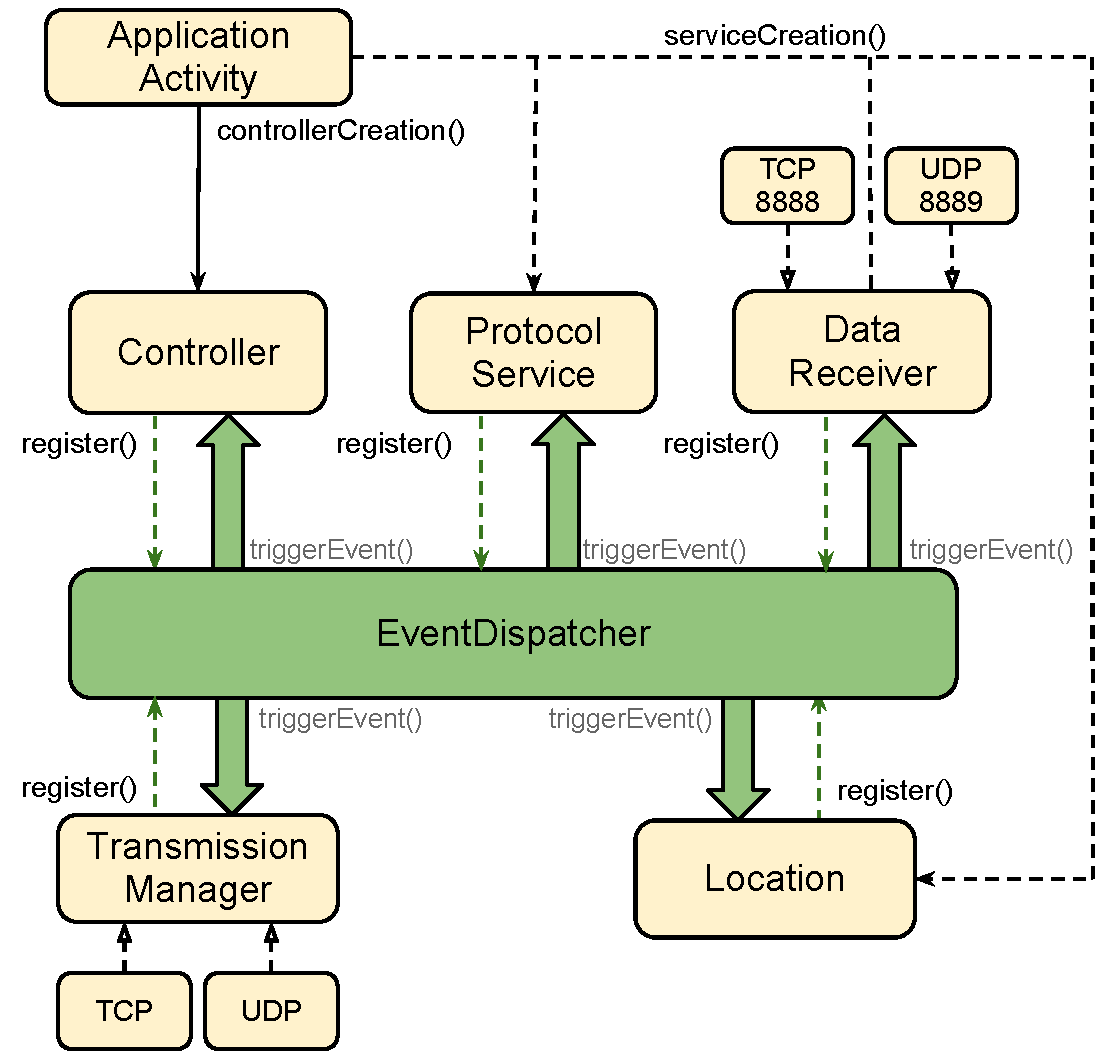
\includegraphics[trim = 10mm 0mm 0mm 0mm,width=3.4in]{imgs/components_architecture.pdf}
	\caption{Graphical representation of a generic Android application structure.}
	\label{fig:architecture}
\end{figure}

Both our frameworks uses the \textit{Event Bus} architectural pattern in order to obtain high decoupling between all the modules. 
They are composed of an \emph{Event Dispatcher} which is responsible of keep track of all the \emph{Components}, registered to listen to specific events, and to use the proper \emph{Component} to handle each triggered \emph{event}, and of the following framework components:
\begin{description}
	\item[\emph{Controller}]  \hfill \\
		It coordinates all the modules the framework provides, managing in fact the lifecycle of every application.
	\item[\emph{Transmission Manager}]  \hfill \\
		Is used to send broadcast, multicast or unicast messages, using a transport level protocol in Android, or using Raw Sockets in Desktop environment.
	\item[\emph{Data Receiver}] \hfill \\
		This module is used to build a Server socket (UDP/TC Socket in Android environment, Data Link Layer Raw Socket in Desktop version) to receive data.
	\item[\emph{Location}] \hfill \\
		Is responsible of positions handling, either interfacing with GPS device or reading fake positions from a text file.  
\end{description}

Given this architecture, changing or adding new modules is as easy as registering them within the \textit{Event Bus} as \textit{Components} listening for needed events. As we can see from figure \ref{fig:architecture}, only a \emph{Protocol service} module and an entry point component (colored in blue) are needed to build a complete testbed application.
%It's worth mentioning that Desktop applications built on top of our framework can use only one type of transmission (Raw Data Link Layer packets), while Android applications can only use TCP or UDP protocols, because of system limitations.
